\chapter{Interface}

\section{Main}

The main page (see Figure \ref{fig:main}) is the page that you see when \PET is loaded. 
Observe that the title displays the default \rel{user} of the tool (``demo'' in this example), as set in the configuration file.

\begin{figure}[h]\label{fig:main}
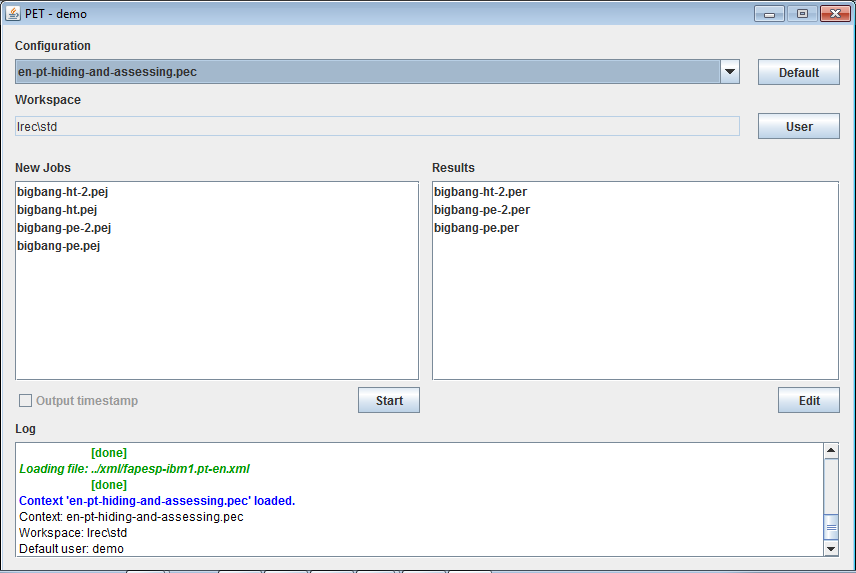
\includegraphics[width=1\textwidth]{img/main}
\caption{\PET's main page}
\end{figure}

Figure \ref{fig:main} shows the following (note that only the relevant elements for this experiment are discussed):

\begin{description}
	\setlength\itemindent{0.5cm}  
	%\item[\tt Configuration] allows the selection of a configuration file, also referred to as \rel{context}, where all the job and interface options are set;
	\item[\tt Workspace] displays the \rel{workspace}, that is, where the files with the jobs to be performed are stored, and where the edited jobs will be saved;
	\item[\tt Jobs] list of available \rel{jobs} (.pej files), i.e. a collection of segments to post-edit or translate;
	\item[\tt Results] list of (partial) \rel{results} (.per files), that is, the output of jobs that have been started (completed or ongoing);
	%\item[\tt Log] lists the progress of actions, such as loading a new \rel{context}, loading dictionaries, etc.;
	%\item[\tt Output timestamp] if set, adds timestamps the \rel{results} files; if not set, a single output file with the same name as the input file will be created, with a different extension;
	%\item[\tt Default] (re-)loads the \rel{default context}, if set in a meta file (see \ref{sec:pec.meta});
	%\item[\tt User] switches to a different \rel{user};
	\item[\tt Start] starts a \rel{job} from zero;
	\item[\tt Edit] continues a (partial) \rel{result};
\end{description}

\textbf{Important}: if you have started a job and done it partially and would like to resume it, then do NOT click ``start'' but click ``edit''. If you do click ``start'' then all your progress in that job so far will be deleted.

%Once one loads the tool using {\tt run.bat} the main page is displayed and a default context is loaded (if specified in a meta file called {\tt pec.meta}).
%Loading a context may take some time and one can visualize the loading progress in the {\tt Log}.
%A context (see \ref{sec:pec}) is a set of parameters that sets \PET to a certain configuration. A valid context is a file ending in {\tt .pec} that necessarily defines a workspace and may define a default user.

%A workspace is a directory in the file system that contains all relevant input and output files.
%Each {\tt user} will have a sub-directory in the workspace tree, so that input and output files are grouped by user.
%If a default user is defined, \PET will load the jobs ({\tt .pej} files) and results ({\tt .per} files) available to that user.
%One can change the user to any of the available ones in the workspace. As for now, \PET does not display the known users, so its up to the user knowing its own username and inputing it correctly when queried.
%If a valid username is given, \PET will update the list of jobs and results according to that user.

\section{Annotation Page}

The annotation page (see Figure \ref{fig:annotation}) is the page that you see when a job is loaded.
%The exact appearance of the annotation page may change due to several aspects of the task (set in the context file).

\begin{figure}[h]\label{fig:annotation}
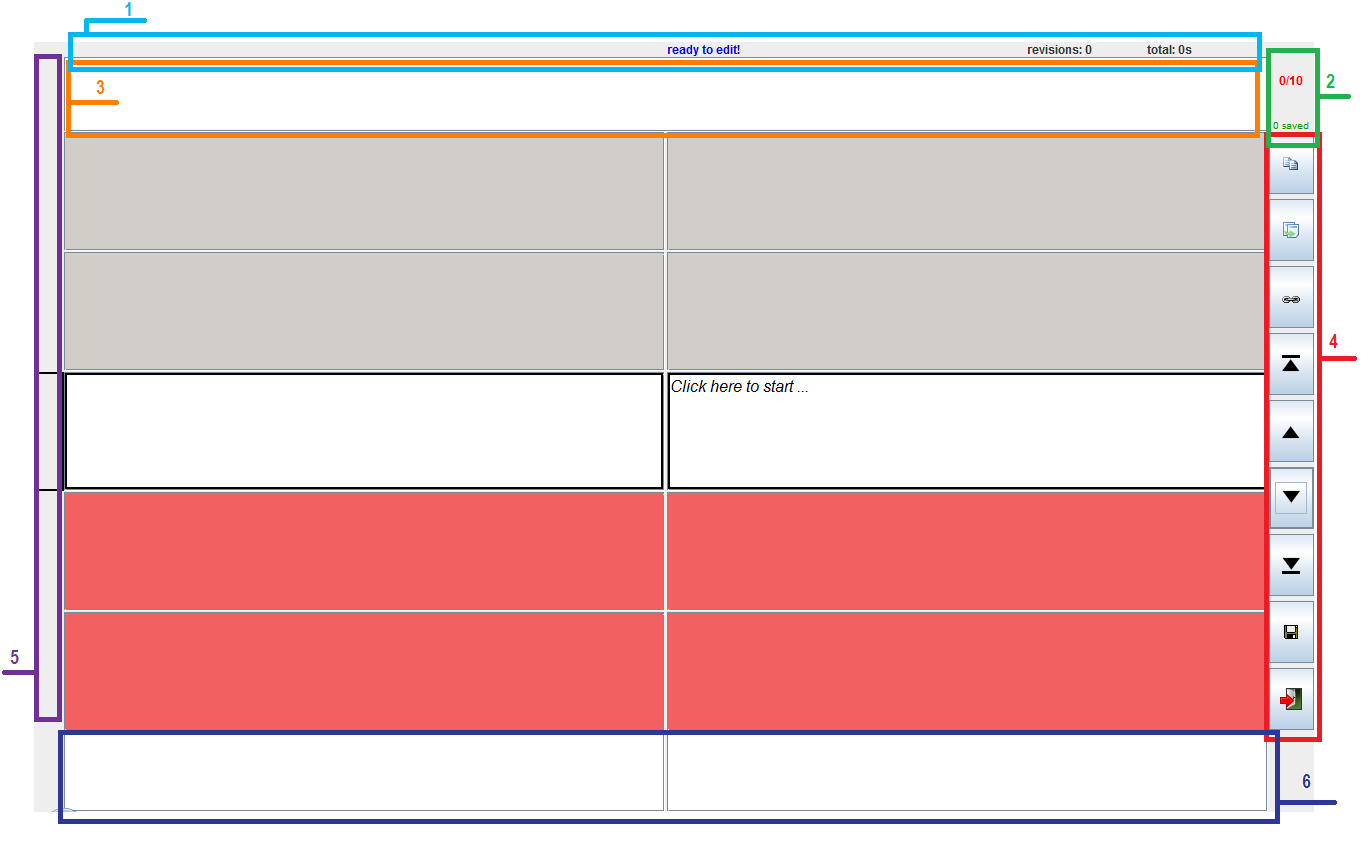
\includegraphics[width=1.0\textwidth]{img/annotation-page-colors}
\caption{\PET's annotation page}
\end{figure}

Figure \ref{fig:annotation} illustrates some important features:

\begin{description}
	\setlength\itemindent{0.5cm}  
	%\item[\tt Top label] the very first line of the page where you will find some useful information on the right, such as the status of the current \rel{unit}, the number of revisions and the time spent on that unit. On the left additional information may be displayed depending on the context;
	\item[\tt Labels (1/light blue)] at the top of the window you will find some useful information, such as the status of the current \rel{unit}, the number of revisions and the time spent on that unit; %. Additional information may be displayed depending on what is set in the context;
	\item[\tt Progress (2/green)] on the top-right hand side. The status of the current job is shown in units done out of the total units in the file (in red); the status of the current jobs is also shown in number of units saved to disk; besides, the timestamp of the last time the progress was saved to disk is shown;
	\item[\tt Top box (3/orange)] displays the source text while the active unit is being post-edited; %the exact text displayed can be chosen by the user by right-clicking on the box. The top box can also used to preview alternative source text, reference text or machine translations;
	\item[\tt Tool box (4/red)] placed on the right-hand-side, it displays action buttons explained in Section \ref{sec:toolbox};
	\item[\tt Id box (5/purple)] placed on the left-hand-side, not used in this experiment; %it is an empty column that may display information such as an identifier or a sequential count for the units on screen;
	\item[\tt Bottom box (6/blue)] not used in this experiment; %displays two panes that render additional information relevant to the active unit; the left pane displays information about the source text and the right pane displays information about the target text (unless \PET's standard orientation is changed via context file);
	\item[\tt Units] the centre of the page contains a grid of 10 lines %(configured via context file) 
	and two columns (i.e for source and translation). The line in the centre of the screen (highlighted with dark borders) is the active unit, as explained in Section \ref{sec:active_unit}.
\end{description}

The top half of the {\tt units} area shows already edited units, while the bottom half shows units to come (see Figure \ref{fig:progress}).
As the user progresses, some units are displayed in green, some are displayed in red. Green stands for ``done'', that is, units that have been post-edited/translated, %/revised, 
while red stands for ``to be done''.
The unit in white is the active unit (always in the central area), and it turns yellow to indicate that the editing has started. Note that the label at the top will change from ``ready to edit'' to ``editing''.
The labels at the top also displays the time spent on the current revision (``partial''), the number of complete revisions (``revisions'') and the total time spent on revisions that are complete (``total'').

\begin{figure}[h]\label{fig:progress}
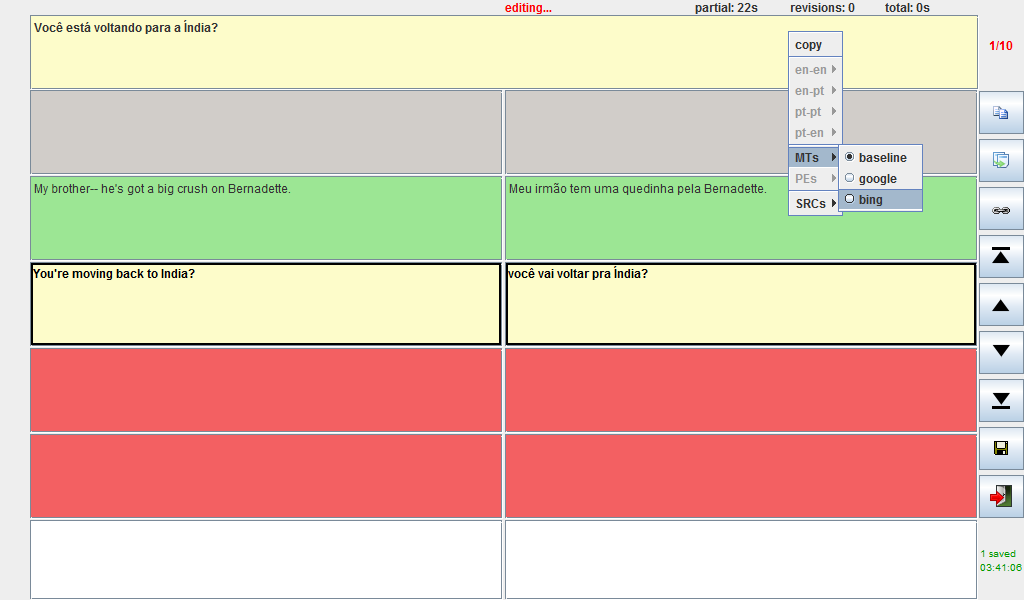
\includegraphics[width=1\textwidth]{img/annotation-progress}
\caption{\PET's annotation page - progress}
\end{figure}

\subsection{Tool box}\label{sec:toolbox}

The context of the tool box (right-hand side box in Figure \ref{fig:progress} with the tool's action buttons) %is also configurable via context file. 
%It generally 
displays:

\begin{description}
	\setlength\itemindent{0.5cm}  
	\item[\tt Copy] not used in this experiment %copy from the top box to the active unit (target side);
	\item[\tt Revert] revert the active unit to its last revision;
	\item[\tt Bind] binds source and target scrolling (useful for long segments);
	\item[\tt Previous undone] searches (backward) for the first undone unit;
	\item[\tt Previous] backs one unit;
	\item[\tt Next] advances one unit;
	\item[\tt Next undone] searches (forward) for the first undone unit;
	\item[\tt Save] saves the current progress to disk;
	\item[\tt Close] closes the job (asks for confirmation and offers a chance to save the progress);
\end{description}

By clicking anywhere on the tool box, it will be focused. Once focused, scrolling down the mouse wheel will move forward and scrolling up will move backward among the units.
When the tool box is focused some shortcuts are available. Placing the pointer over a button for a second will show a tool tip text and information about shortcuts for that button.

Shortcuts are not case-sensitive, some of them are:
\begin{description}
	\setlength\itemindent{0.5cm}  
	\item[\tt I] enables the \textit{insert} mode, that is, it changes the active unit to the ``editing'' state;
	%\item[\tt $<$ALT$>$+$\downarrow$] moves to next unit (if editing state);
	%\item[\tt $<$ALT$>$+$\uparrow$] moves to previous unit (if editing state);
	\item[\tt $\downarrow$] moves to next unit (if in scrolling state);
	\item[\tt $\uparrow$] moves to previous unit (if in scrolling state);
	\item[\tt $<$END$>$] moves forward until an undone unit is found;
	\item[\tt $<$HOME$>$] moves backward until an undone unit is found;
	\item[\tt B] binds source and target scrolling;
	\item[\tt $<$F10$>$] saves;
	\item[\tt $<$ALT$>$+$<$F4$>$] closes the tool;
\end{description}


\subsection{Active unit}\label{sec:active_unit}

The active unit is the central line in the units area.
It is highlighted by a dark border and is the only unit whose target side is editable.
By default, the active unit is in the state ``ready to edit'', when its target box receives the focus the unit will go to the state ``editing'' (the box turns yellow), which means that effort indicators will start to be logged.
The active unit in the ``editing'' state will be generally referred to as the \rel{editing box}.

The \rel{editing box} offers some shortcuts, some of them are:

\begin{description}
	\setlength\itemindent{0.5cm}  
	\item[\tt $<$ALT$>$+$\downarrow$] finalizes the current unit and moves to next unit;
	\item[\tt $<$ALT$>$+N] finalizes the current editing and moves forward starting with the next unit;
	\item[\tt $<$ALT$>$+$\uparrow$] finalizes the current unit and moves to previous unit;
	\item[\tt $<$ALT$>$+P] finalizes the current unit and moves backward starting with the previous unit;	
	\item[\tt $<$ALT$>$+B] binds source and target scrolling;
	\item[\tt $<$CTRL$>$+Z] undo editing;
	\item[\tt $<$CTRL$>$+Y] redo editing;
	\item[\tt $<$CTRL$>$+C] copy selection;
	\item[\tt $<$CTRL$>$+X] cut selection;
	\item[\tt $<$CTRL$>$+V] paste;
	\item[\tt $<$CTRL$>$+R] replace/insert selection;
	\item[\tt $<$CTRL$>$+I] insert/replace selection;
	\item[\tt $<$CTRL$>$+D] delete selection;
	\item[\tt $<$CTRL$>$+S] shift selection;
\end{description}

In case a unit is in the state ``editing'' an attempt to close the job will result in a prompt to finalize or discard the modifications done to that active unit. 

%\fixme{Edited units are saved once they are completed.  - ta certo isso que adicionei, ne? -- Depende, "save to disk"? dai depende do "autoSave"}

%\subsection{Drop-down menu}\label{sec:menu}
%
%By right-clicking the several text boxes one gets a drop-down menu with a few options.
%All the boxes, except for the active unit, are read-only, therefore they will simply display read-only options, such as ``copy'' and dictionary lookup. The options available will depend on what is given to the tool as input for the job (dictionaries, alternative translations, etc.).
%
%Available dictionaries are shown using the languages of the current job, for instance: source-source or target-target (monolingual dictionaries), source-target or target-source (bilingual dictionaries).
%Several dictionaries can be loaded and lookup operations are grouped by dictionary (see Figure \ref{fig:dictionary}). In order to use dictionaries, it is necessary to right-click a portion of the text, as opposed to simply clicking the unit box. 
%In the \rel{editing box}, selecting an option from a dictionary will replace the selected text by the selected option.
%
%Alternative text can be displayed for the active unit in the ``editing'' state if such alternative text is given in the {\tt .pej} file \ref{sec:pej}.
%Alternative text includes: i) multiple sources, ii) multiple references and iii) multiple translations. Past revisions of the unit (PEs) can also be shown and used, if they are available for the job.
%The drop down menu displays these alternative texts.
%
%Moving the mouse over the options will display a preview on the top box, while selecting one of the options will cause the alternative text to replace the content of the current box.
%One may replace a source by an alternative source, the top box by any of the available alternative text and the target unit by an available translation (MT or PE).
%
%\begin{figure}[h]\label{fig:dictionary}
%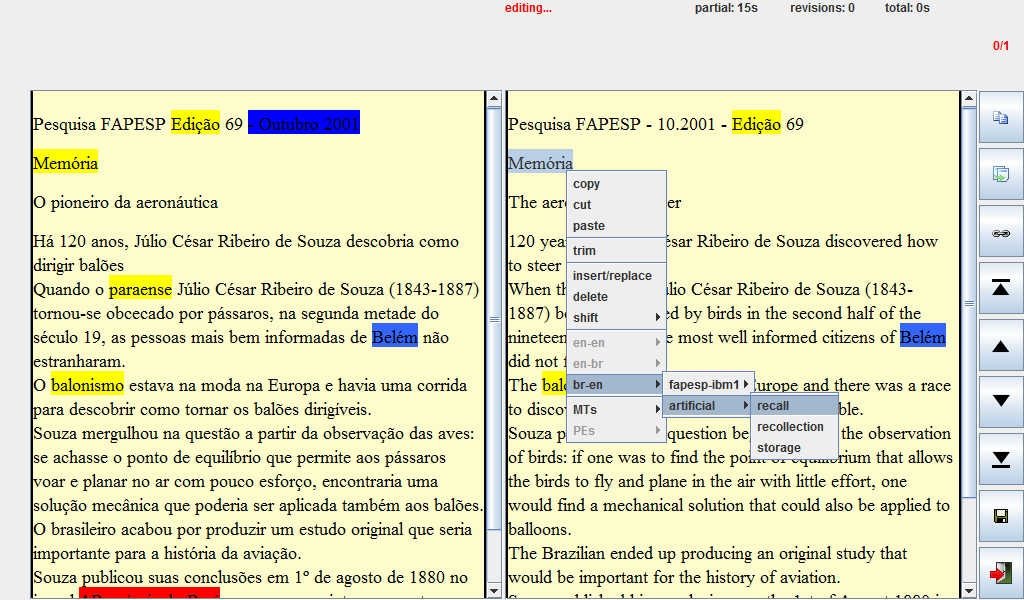
\includegraphics[width=1\textwidth]{img/annotation-dictionary}
%\caption{\PET's annotation page - dictionaries}
%\end{figure}

\subsection{Drag and drop}\label{sec:dragdrop}

Text can be dragged from any text box (source, target, etc.) and dropped into the active unit's target box (if ``editing'').
Text can also be moved around within the editing box by using drag and drop.

%\section{Assessment Page}
%
%An optional assessment page can be displayed after every active unit is completed.
%The exact type of assessment can be configured via context file.
%Figures \ref{fig:assessment} and \ref{fig:assessment-multiple} show examples, the latter displays a query that accepts multiple answers.
%
%\begin{figure}[h]\label{fig:assessment}
%\center
%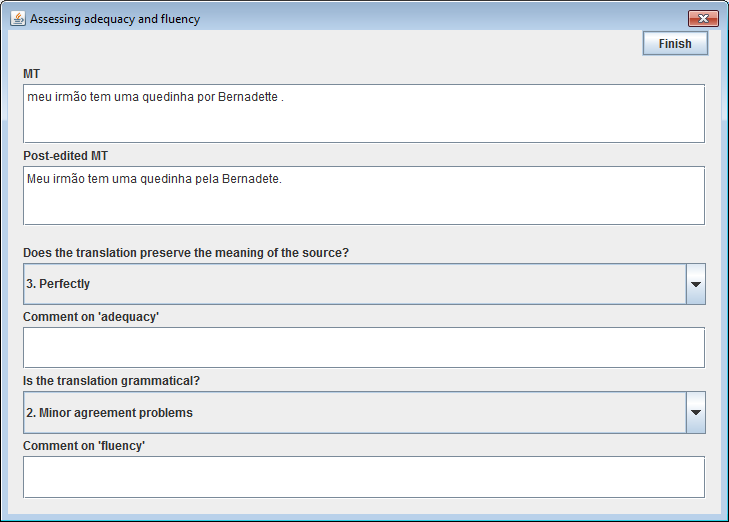
\includegraphics[width=0.75\textwidth]{img/assessment-page}
%\caption{\PET's assessment page - single selection}
%\end{figure}
%
%\begin{figure}[h]\label{fig:assessment-multiple}
%\center
%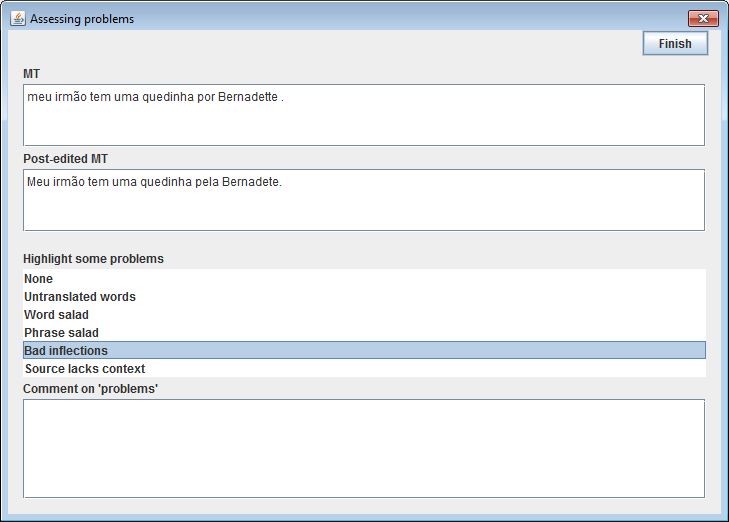
\includegraphics[width=0.75\textwidth]{img/assessment-page2}
%\caption{\PET's assessment page - multiple selection}
%\end{figure}
%
